\section{Shape variations in the fit}
\label{ref:fit:var}

In \HistFactory, fit templates are allowed to have coherent shape variations.
For a single bin, the yield after variation is defined as:

\begin{equation}
    n_\text{var} = n_\text{nom} + \sum_i f_i(n_+, n_-, n_\text{nom}, \alpha)
\end{equation}
where $n$ denote yields in a single bin, and
$n_+, n_-$ are the yields when the variation $\alpha$ is at $\pm 1$.
$f$ is the interpolation/extrapolation function to specify variation
at any value;
only piecewise-linear and quadratic-interpolation-linear-extrapolation
in the \HistFactory are used.
The \emph{coherence} comes from the fact that the $\pm 1$ yields need to be
specified for \emph{all} bins at once, in the form of histograms.

The template variations employed in this analysis are listed in the following
paragraphs.

\subsection{Form factor uncertainties}

To take form factor uncertainties into account, the correlation
matrices of the form factor parameters are transformed
according to \cref{appx:ff-var}, which produces $\pm 1\sigma$ variations
in an orthonormal error eigen basis.

Additional fit templates are generated by reweighting MC samples at the
variations and are included in the fit.
A sample $\pm 1\sigma$ variation of the \Dz\mun templates is listed in
\cref{fig:fit-variations:ff}.

\begin{figure}[htb]
    %\begin{subfigure}{\textwidth}
    %    \caption{
    %        $\Bm \rightarrow \Dz\taum\neutb$ vs.
    %        $\Bzb \rightarrow \Dstarp\taum\neutb$.
    %    }
    %    \label{fig:d0-sig-vs-dst-sig}
    %\end{subfigure}

    \caption{
        \Dz\mun nominal and $\pm 1\sigma$ variation templates for
        parameter $u_1$, which is mostly aligned with
        some param in the BGL parameterization.
    }
    \label{fig:fit-variations:ff}
\end{figure}


\subsection{Data-driven Dalitz-inspired deformations to $DDX$ model}
\label{ref:fit:var:ddx}

The $DDX$ are poorly understood and the phase space model are known to be
unphysical but no better model is available.
Additional variations are introduced to give more freedom to the fit variables,
allowing for a data-driven approach for the determination of $DDX$ decays.

The variations are inspired by Dalitz plots, where a single scaler decays into
three scaler, and the phase space is uniquely determined by two variables.
Here the invariant mass of $DD$ is chosen as the proxy to deform the phase
space linearly and quadratically, as defined in EQN.


\subsection{\Kstar weight up/down in $DDX$ templates}

An $DDX$ event is considered to contain a \Kstar if
$(p_B - p_{D_\text{1st}} - p_{D_\text{2nd}})^2 > 680$ MeV.
The \Kstar events are weighted up (to 2) and down (to 0) to allow additional
variations for the $DDX$ templates, because the
branching fraction of \Kstar is not precisely known.


\subsection{Data-driven phenomenological deformation to $D_H^{**}$ model}

The $D_H^{**}$ MC samples are generated with ISGW2 form factor model, which
is known to be insufficient in describing data:
Similar to run 1 analysis, the \qSq in the 2OS sample fits poorly with the ISGW2
model.
A deformation based on the true \qSq
in $D_H^{**}$ is introduced to provide more freedom in fit variables,
allowing for a data-driven approach to determine the shapes of these modes.
A comparison between nominal and variated $D_H^{**}$ templates can be seen at.


\subsection{Effect of kaon, pion decay-in-flight in muon misID template}
\label{ref:fit:var:misid-dif}

\kaon and \pion have some probability of decay to a \muon between upstream and
downstream tracking (decay-in-flight, DiF),
which leads to a mis-measurement of the track momentum,
and authentic signals in the muon stations.
In our fake \muon sample, however, only events \emph{without} any \muon
signal are selected, thus \emph{none} of the mis-identified \kaon and \pion has
the DiF effect.

To account for the DiF effect, we use a smearing approach on top of the
unfolding described in \cref{ref:fit:tmpl:misid}:

\begin{enumerate}
    % FIXME: Find the MC sample ID and regenerate for run 2!
    \item Select $K, \pi$ passing truth-matching and nominal $\mu$ selection
        requirements from a MC sample.

    \item Find the true and reconstructed momenta of
        $K, \pi$.
        Use ratios of
        $\text{smear factor}_i \equiv \frac{\text{reco}_i}{\text{true}_i}$
        as the smearing factor for the $i$-component of the 3-momentum,
        with the assumption that MC models DiF sufficiently correctly.

    \item Put all smearing factors in an array,
        and for the fake \muon track of each misID event,
        randomly select one to smear the reconstructed momentum:

        \begin{equation}
            p_{i,\text{smeared}} =
                p_{i,\text{reco}} \times \text{smear factor}_i
        \end{equation}

    \item Estimate the $B$ meson rest frame momentum with the rest frame
        approximation technique. % FIXME: Citation?
    \item Recompute fit variables
        $\{\mmSq, \qSq, \el\}_K, \{\mmSq, \qSq, \el\}_\pi$
        with the new fake \muon track momentum.
        These sets of variables will be refer as $K$-smeared and $\pi$-smeared.
\end{enumerate}

When building the fit variable templates, for each event of tagged species
$\hat{t}'$,
the nominal fit variables $\{\mmSq, \qSq, \el\}$ and the two sets of the smeared
fit variables are weighted according to the following rules:

\begin{itemize}
    \item $K$-smeared: \misEff[\hat{t}']{K}
    \item $\pi$-smeared: \misEff[\hat{t}']{\pi}
    \item Nominal: $1 - \misEff[\hat{t}']{K} - \misEff[\hat{t}']{\pi}$
\end{itemize}
where the efficiencies are obtained from the unfolding procedure.
A comparison between unsmeared and smeared misID fit variables is shown
in \cref{fig:unfolding-fit-vars-smear}.
\techlink{appx:tech:apply-misid-dif-weights}

% Generated in /lhcb-ntuples-gen/studies/plot-RDX_misid_unfold_fit_vars, by
% running the script gen.sh inside
\begin{figure}[htb]
    \centering
    \begin{subfigure}[b]{0.32\textwidth}
        \centering
        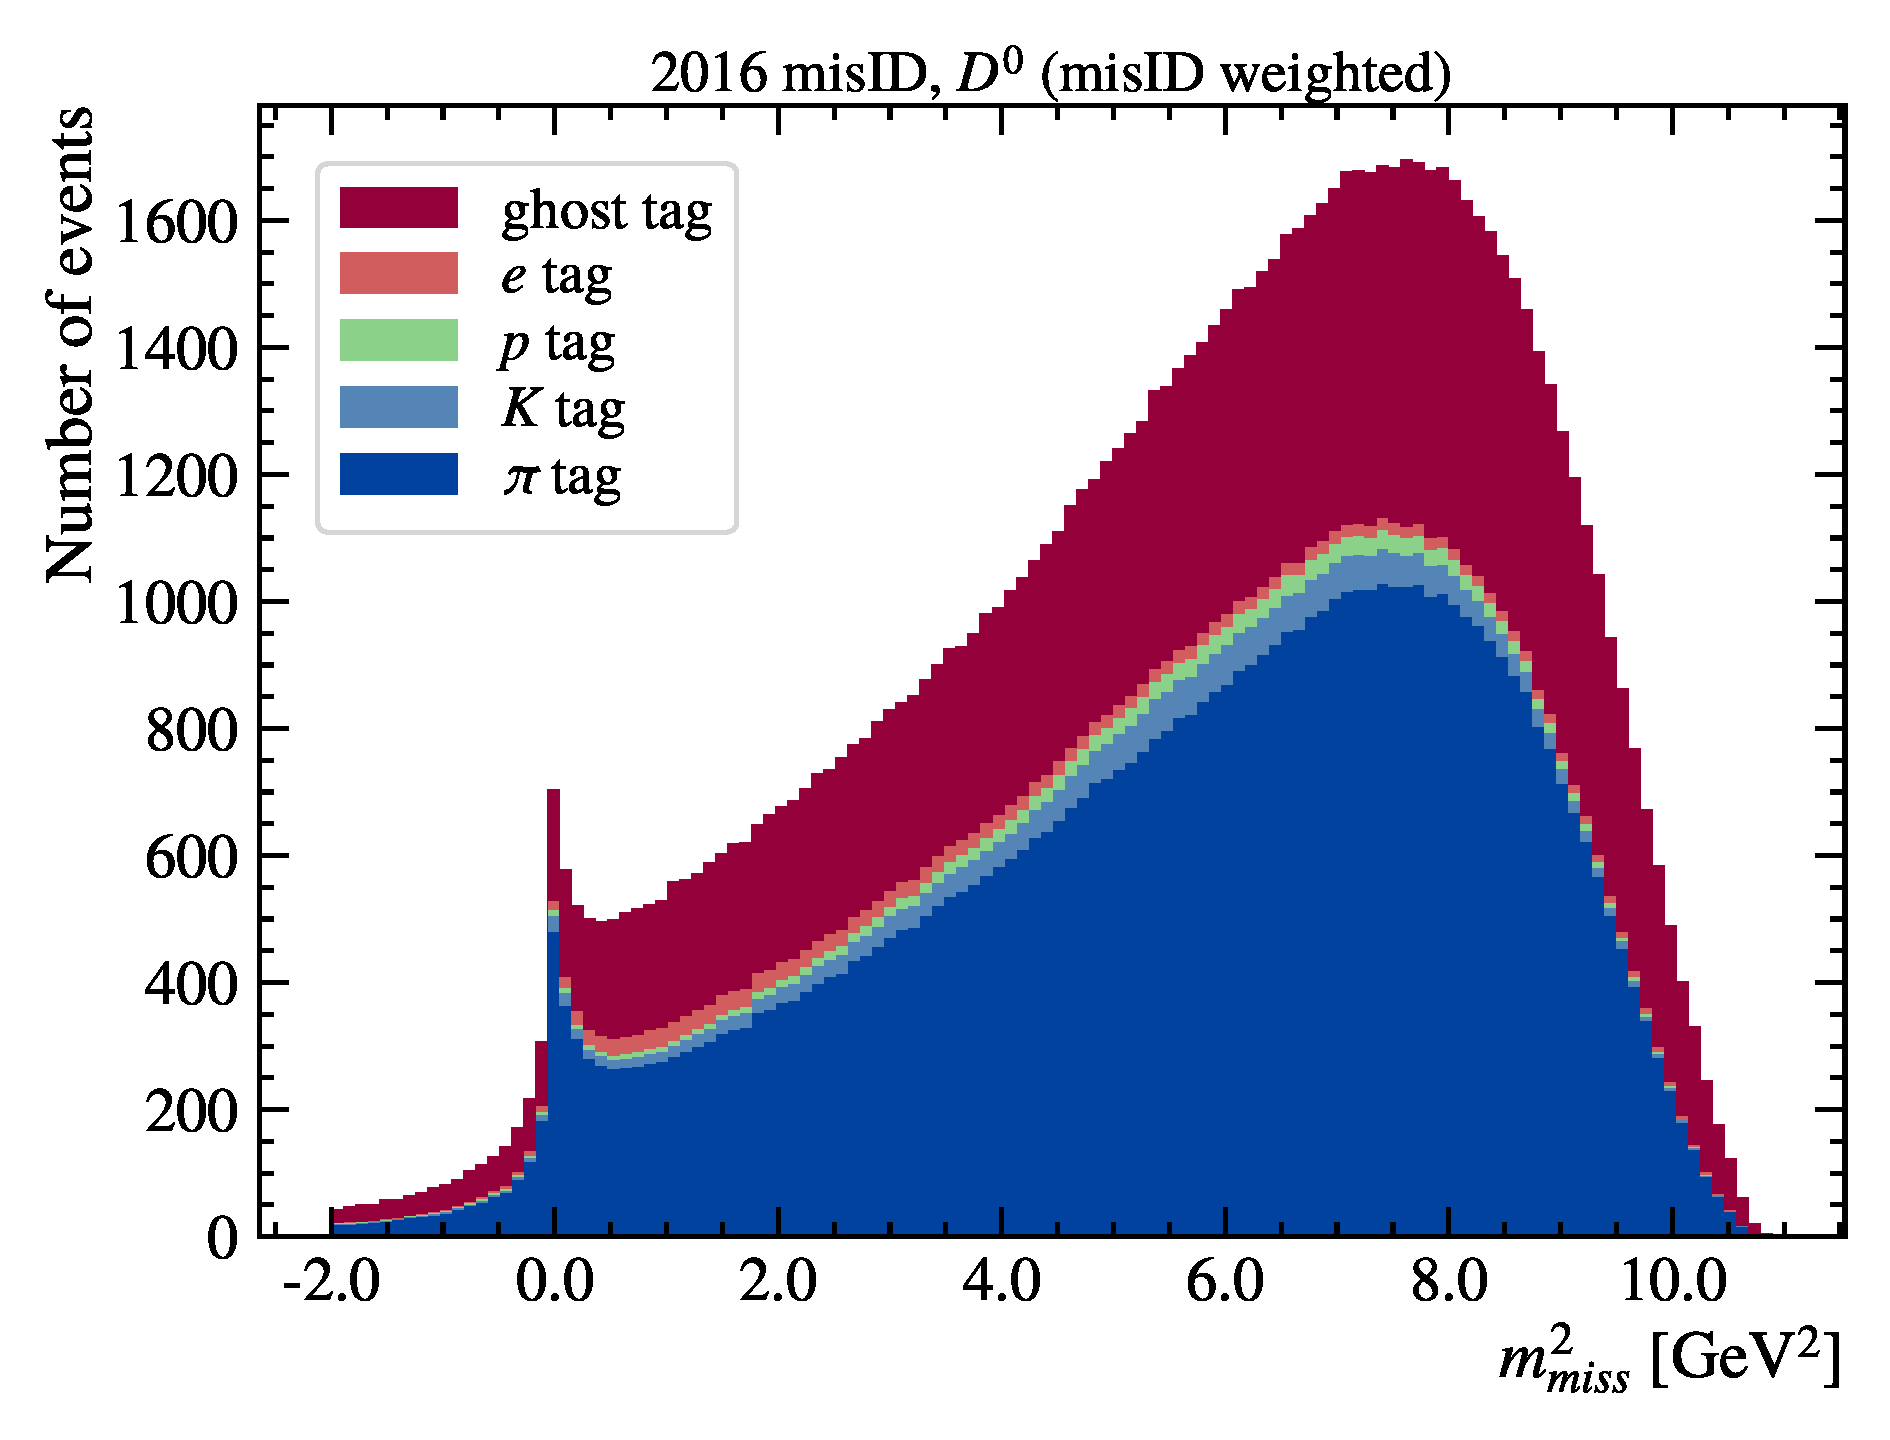
\includegraphics[width=\textwidth]{figs-fit-fit-templates/data-driven-plots/misid/D0_mm2.pdf}
    \end{subfigure}
    \hfill
    \begin{subfigure}[b]{0.32\textwidth}
        \centering
        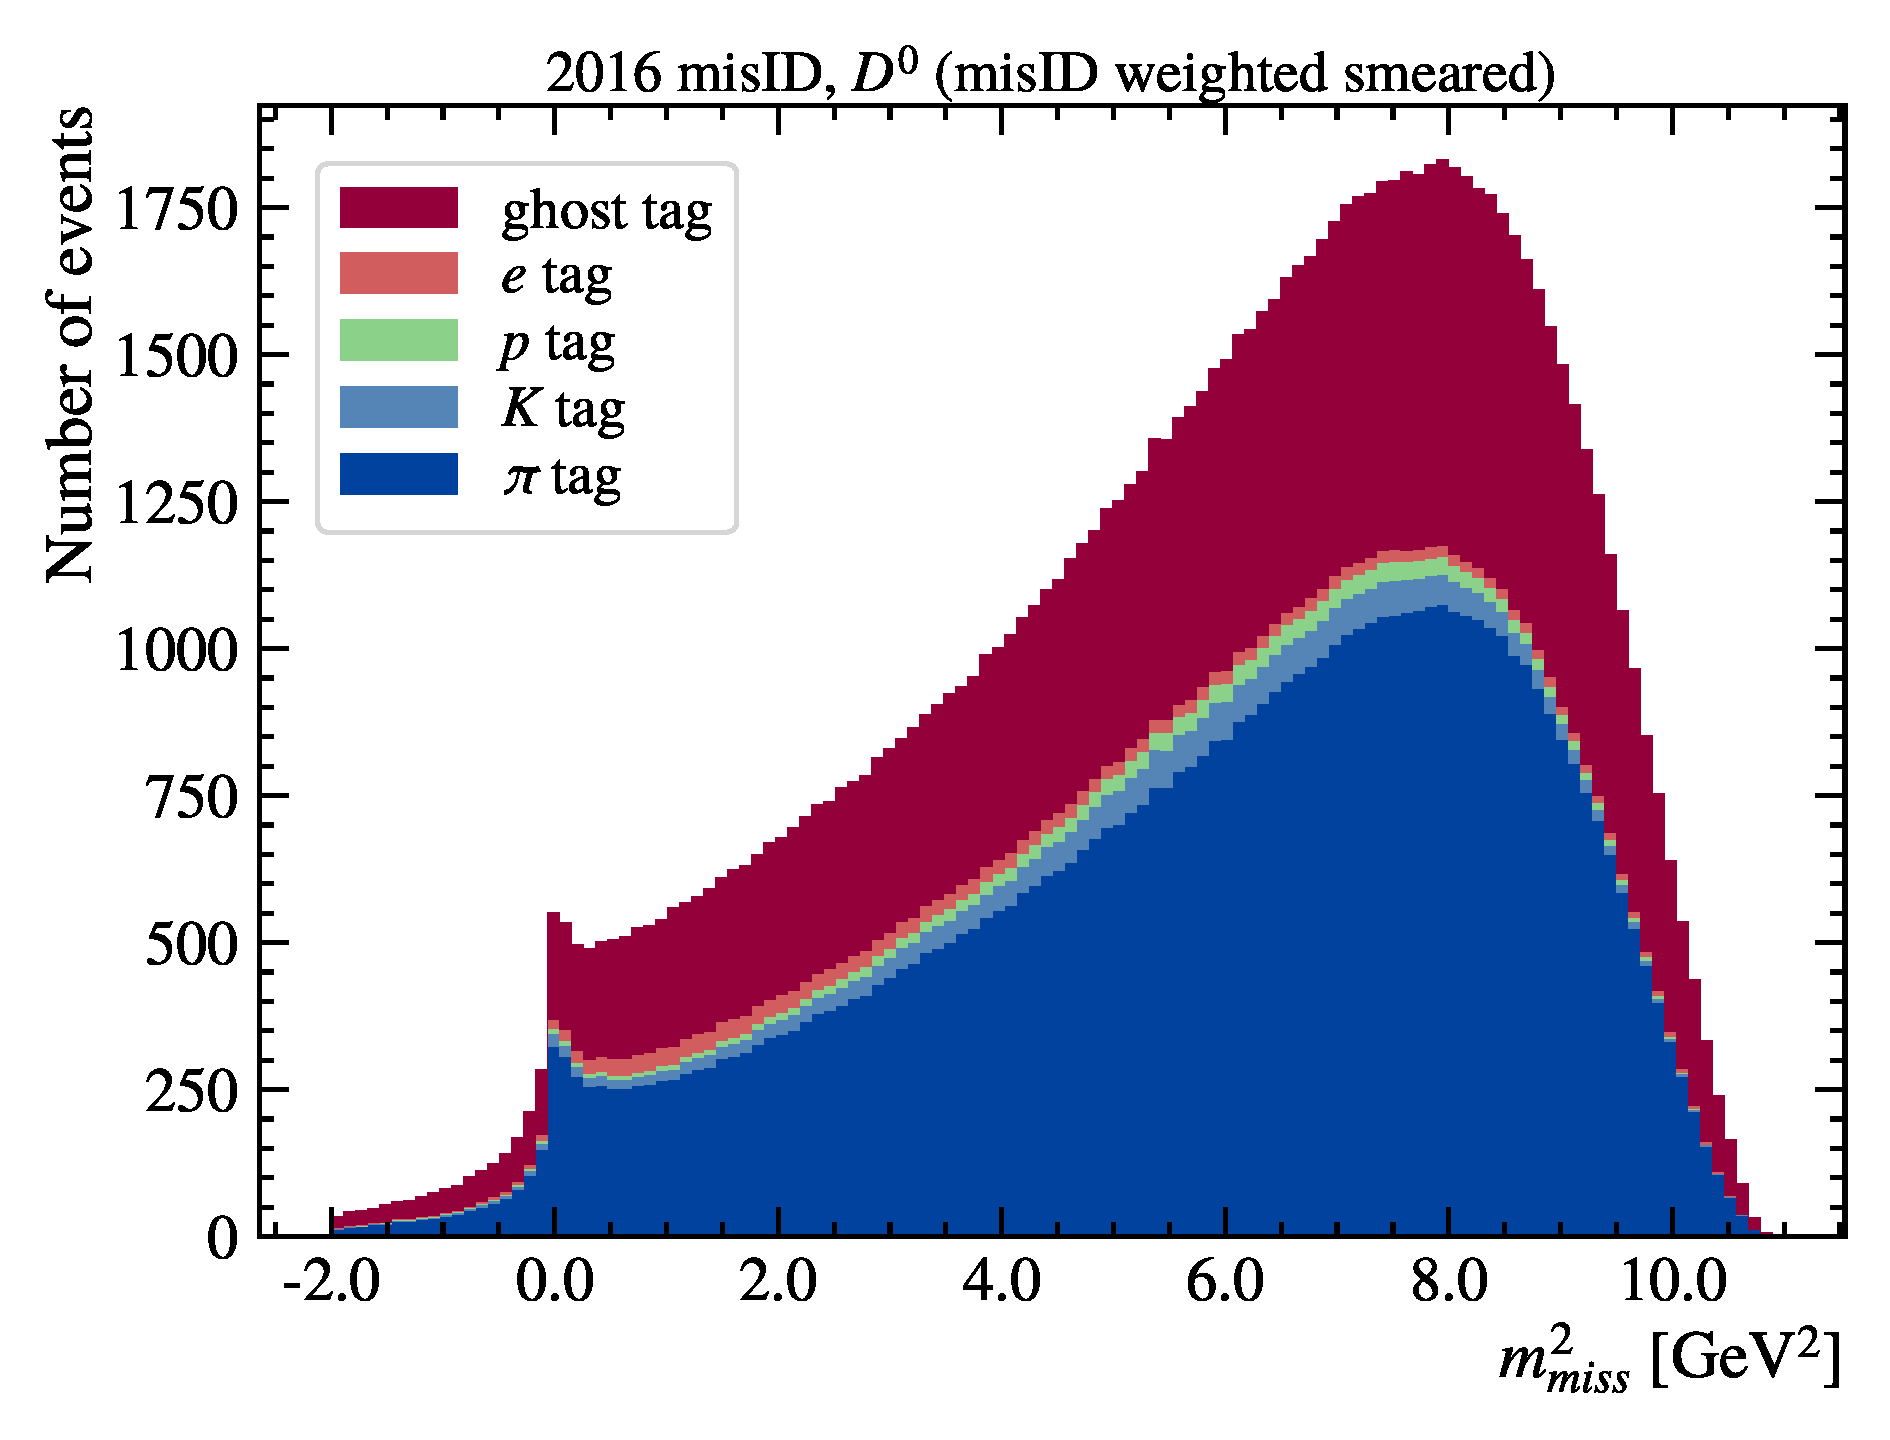
\includegraphics[width=\textwidth]{figs-fit-fit-templates/data-driven-plots/misid/D0_mm2_smr.pdf}
    \end{subfigure}
    \hfill
    \begin{subfigure}[b]{0.32\textwidth}
        \centering
        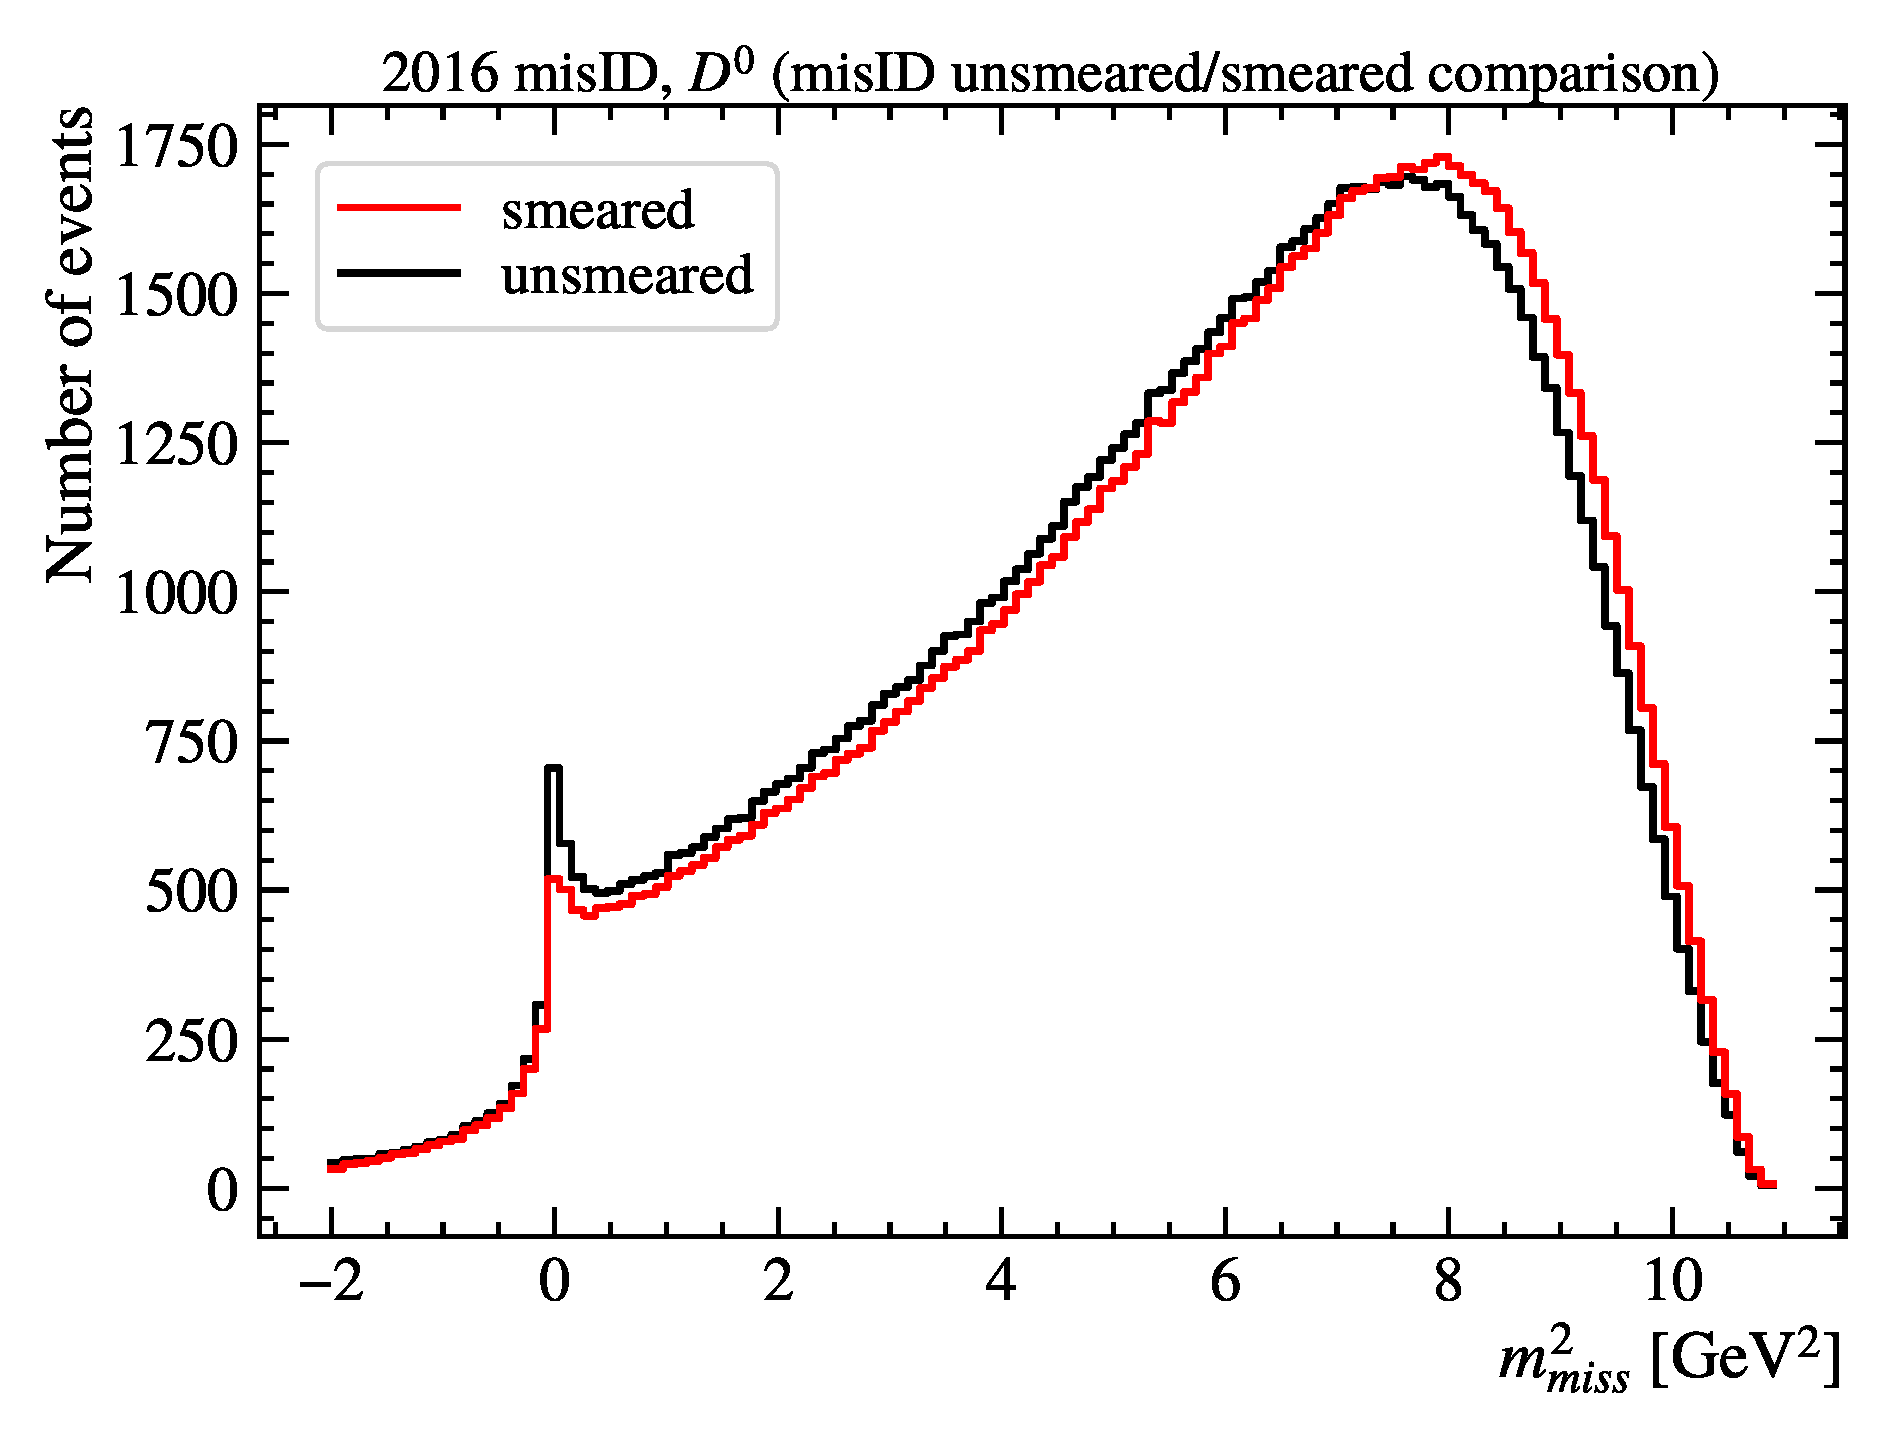
\includegraphics[width=\textwidth]{figs-fit-fit-templates/data-driven-plots/misid/D0_mm2_comp.pdf}
    \end{subfigure}
    \\
    \begin{subfigure}[b]{0.32\textwidth}
        \centering
        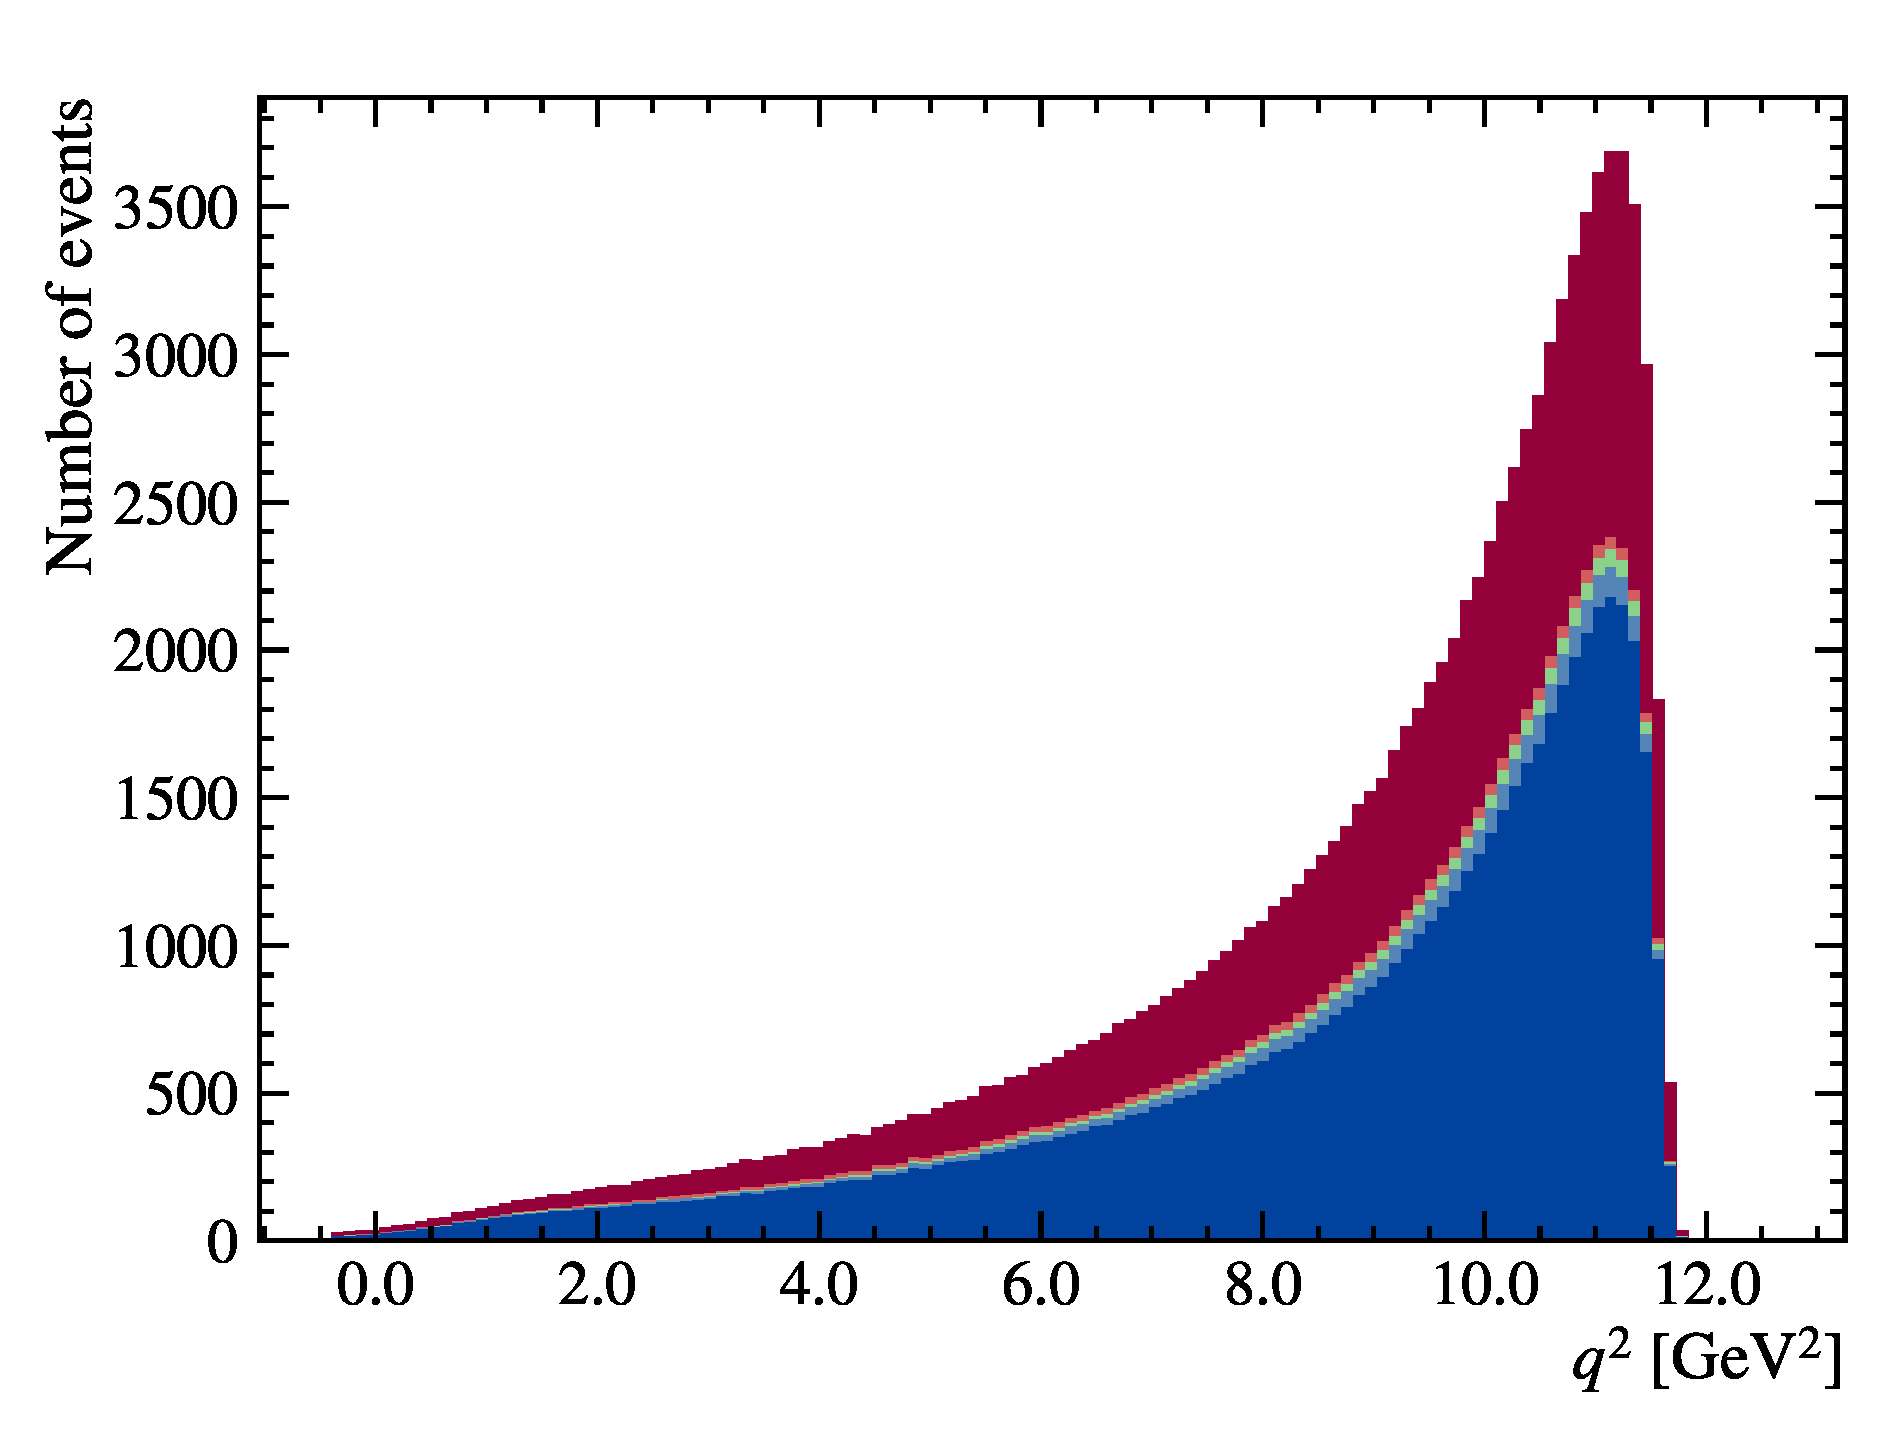
\includegraphics[width=\textwidth]{figs-fit-fit-templates/data-driven-plots/misid/D0_q2.pdf}
    \end{subfigure}
    \hfill
    \begin{subfigure}[b]{0.32\textwidth}
        \centering
        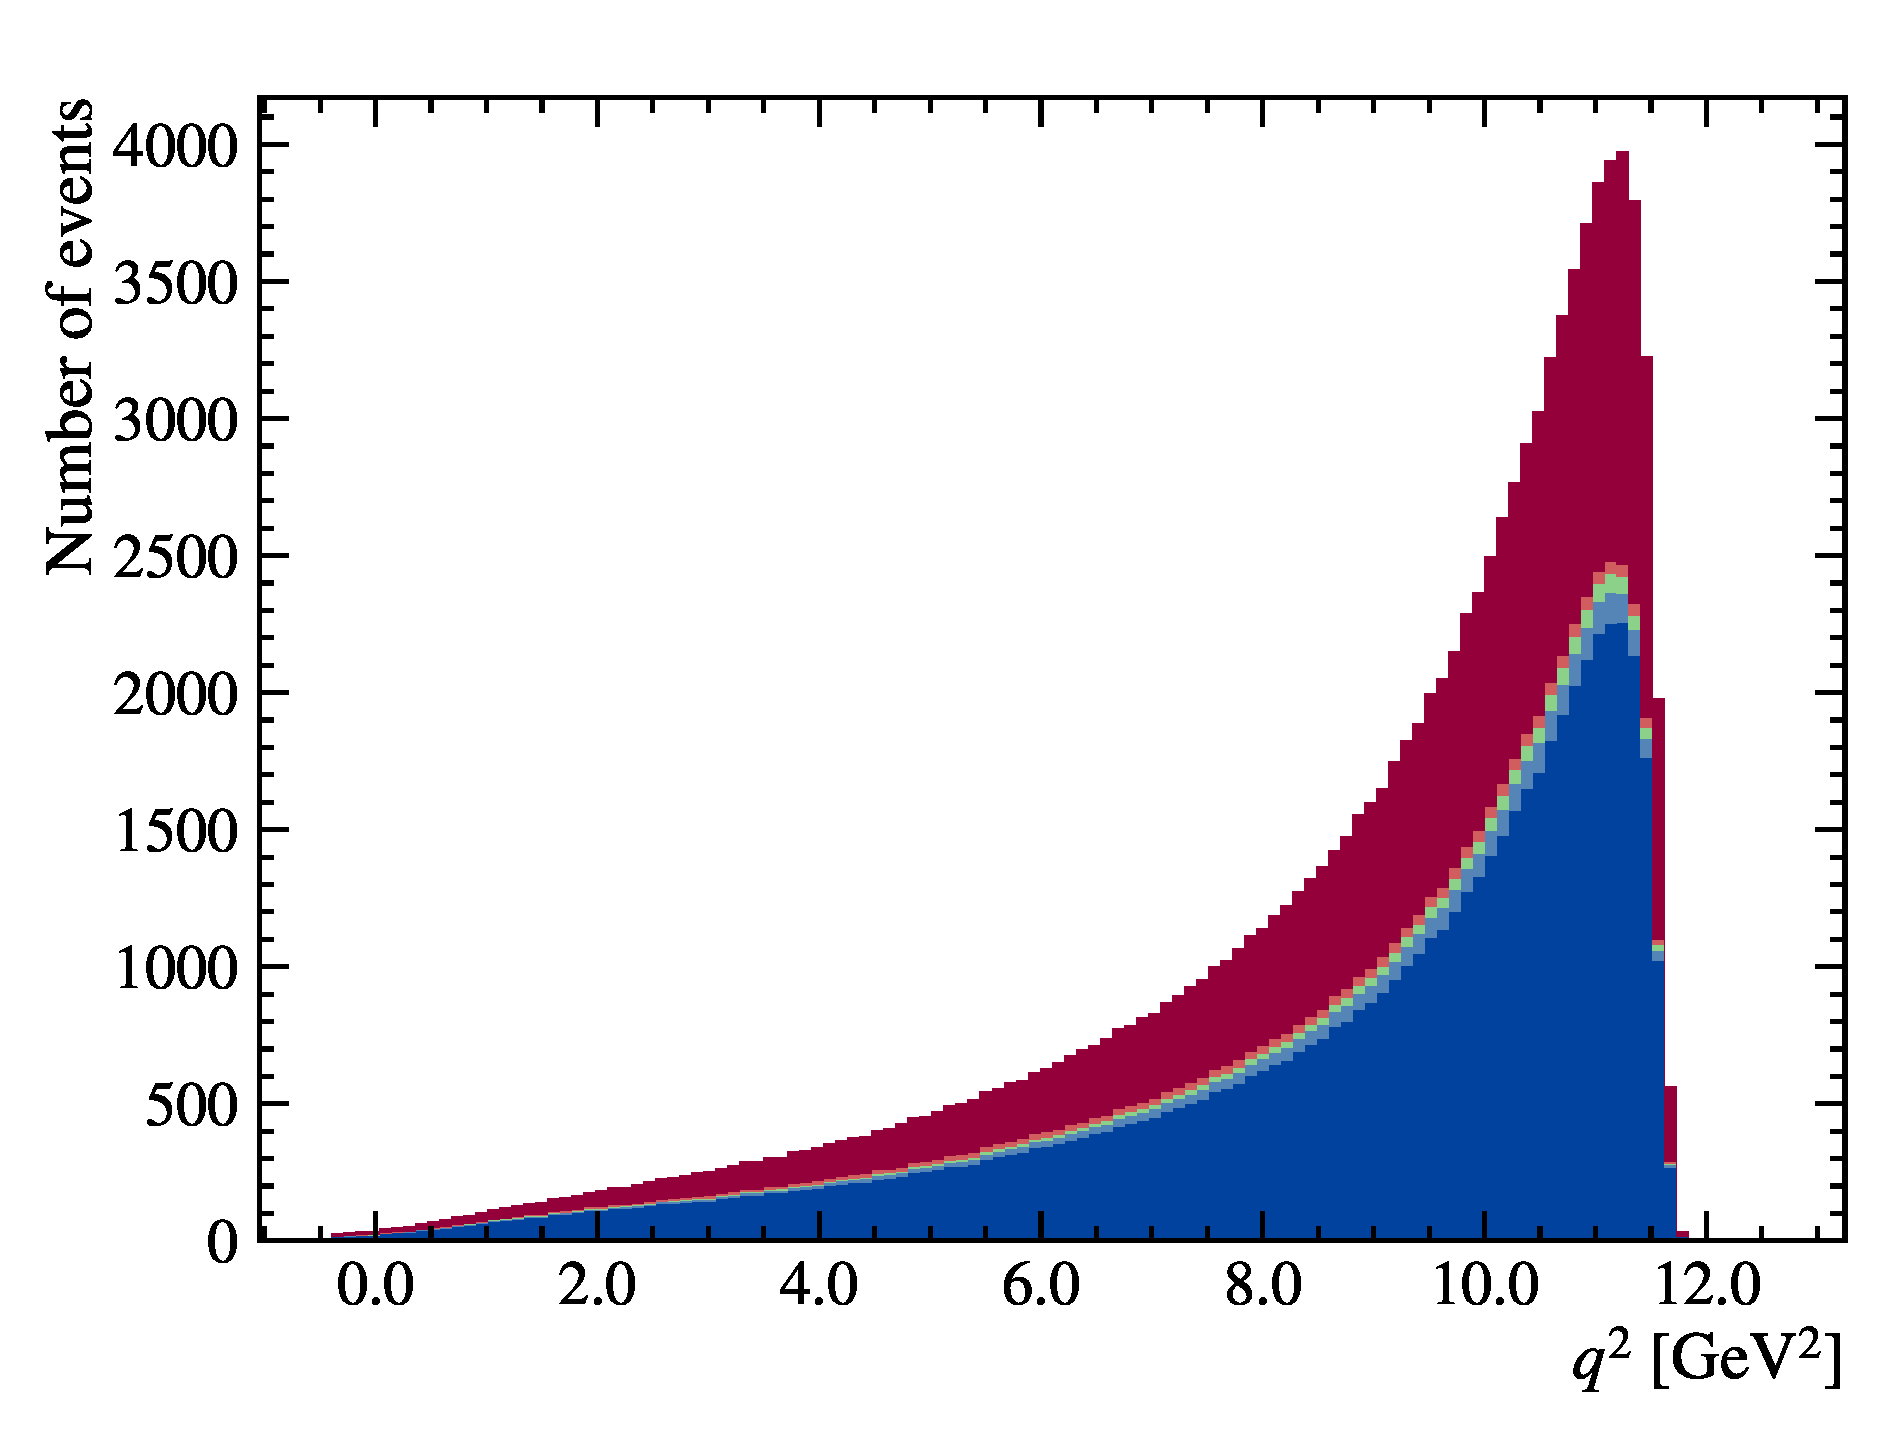
\includegraphics[width=\textwidth]{figs-fit-fit-templates/data-driven-plots/misid/D0_q2_smr.pdf}
    \end{subfigure}
    \hfill
    \begin{subfigure}[b]{0.32\textwidth}
        \centering
        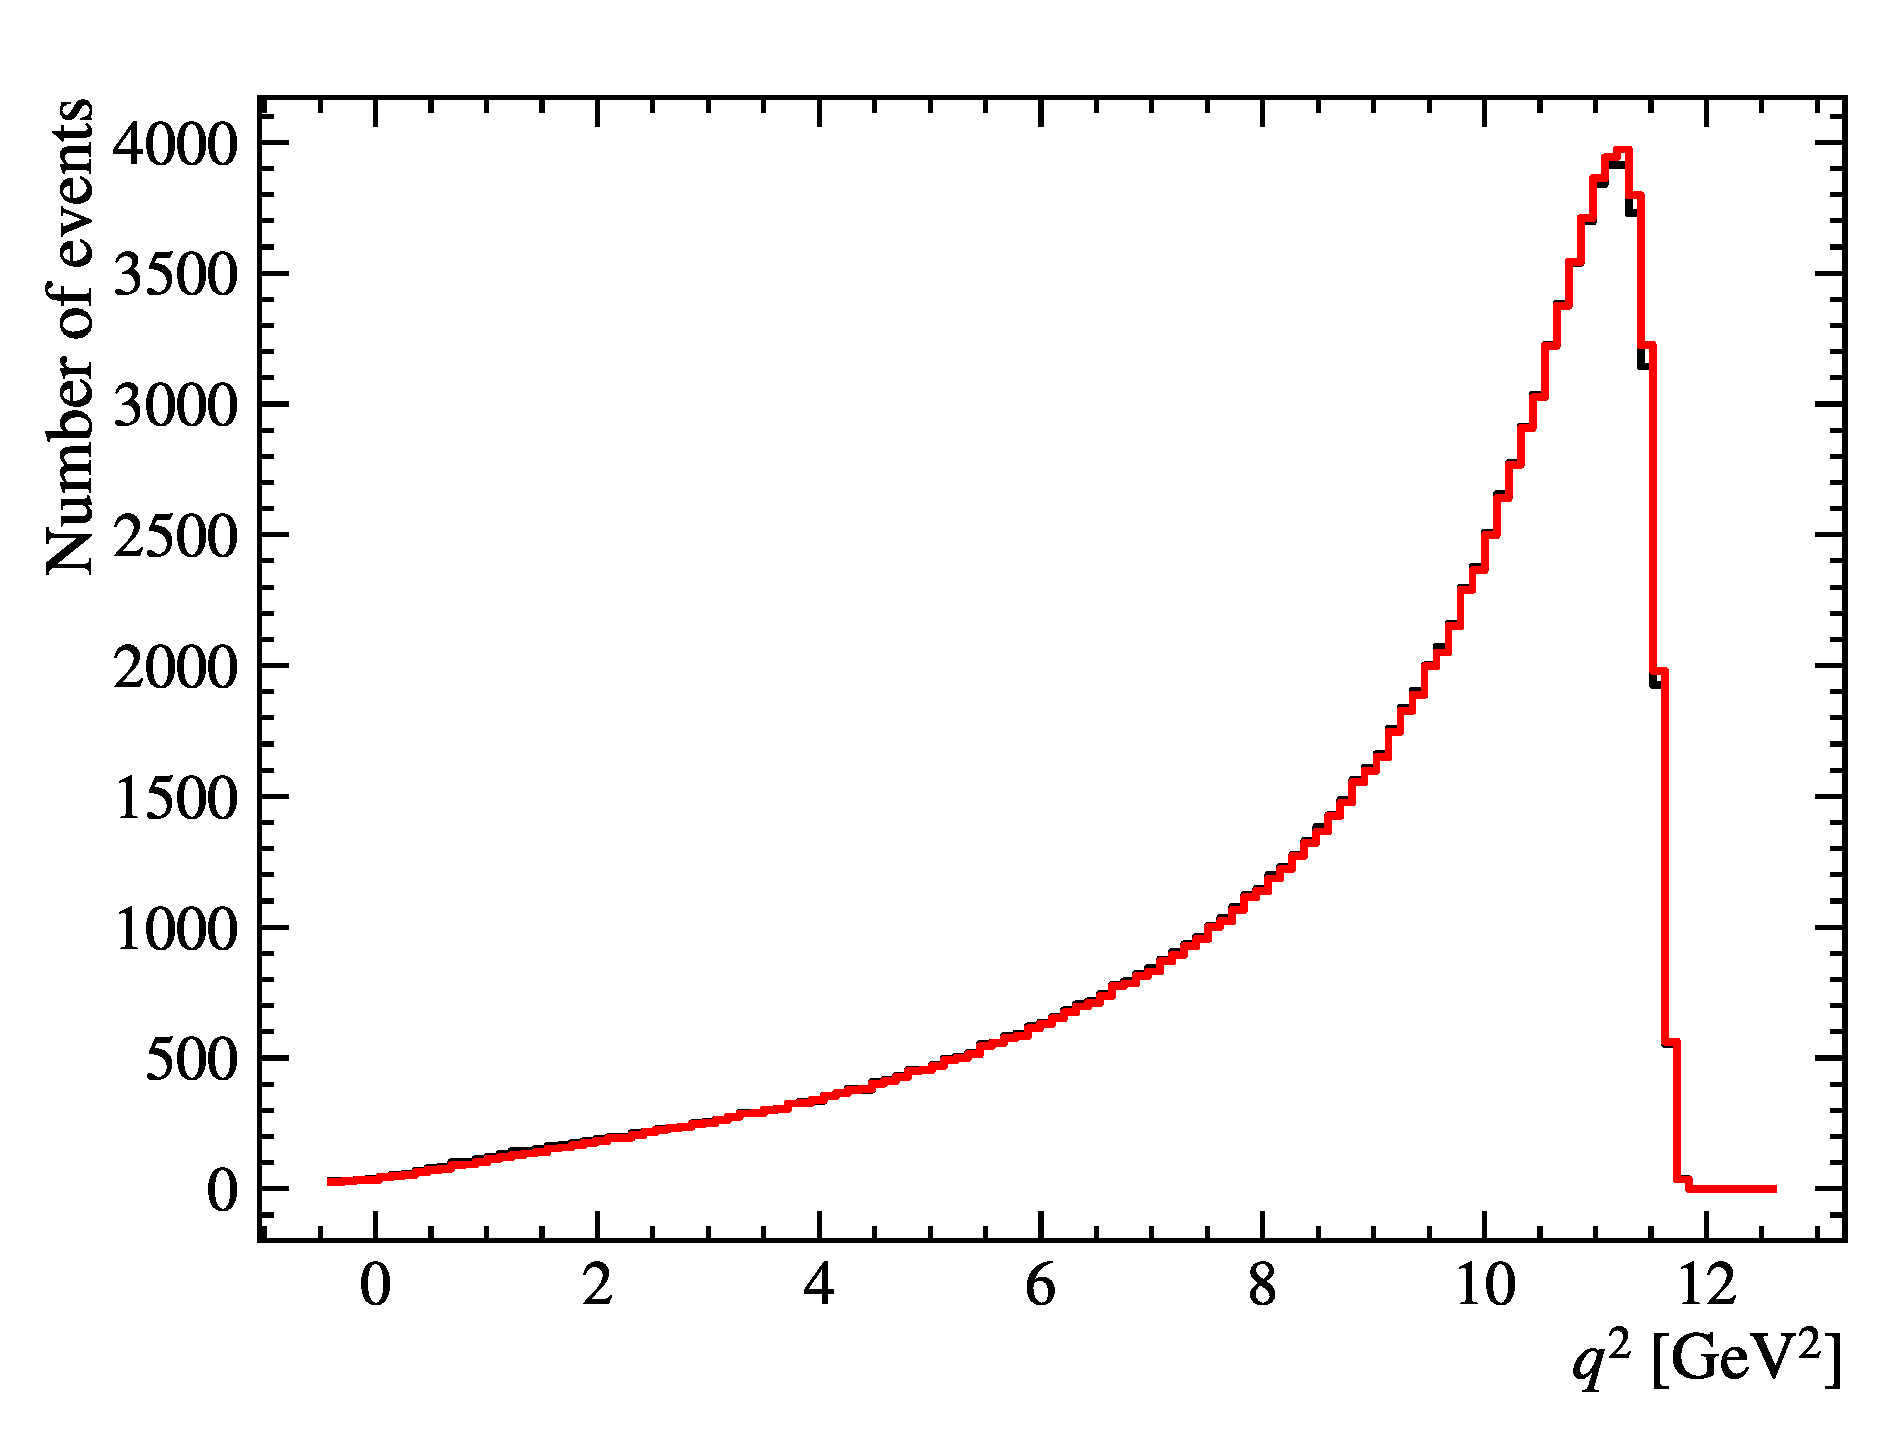
\includegraphics[width=\textwidth]{figs-fit-fit-templates/data-driven-plots/misid/D0_q2_comp.pdf}
    \end{subfigure}
    \\
    \begin{subfigure}[b]{0.32\textwidth}
        \centering
        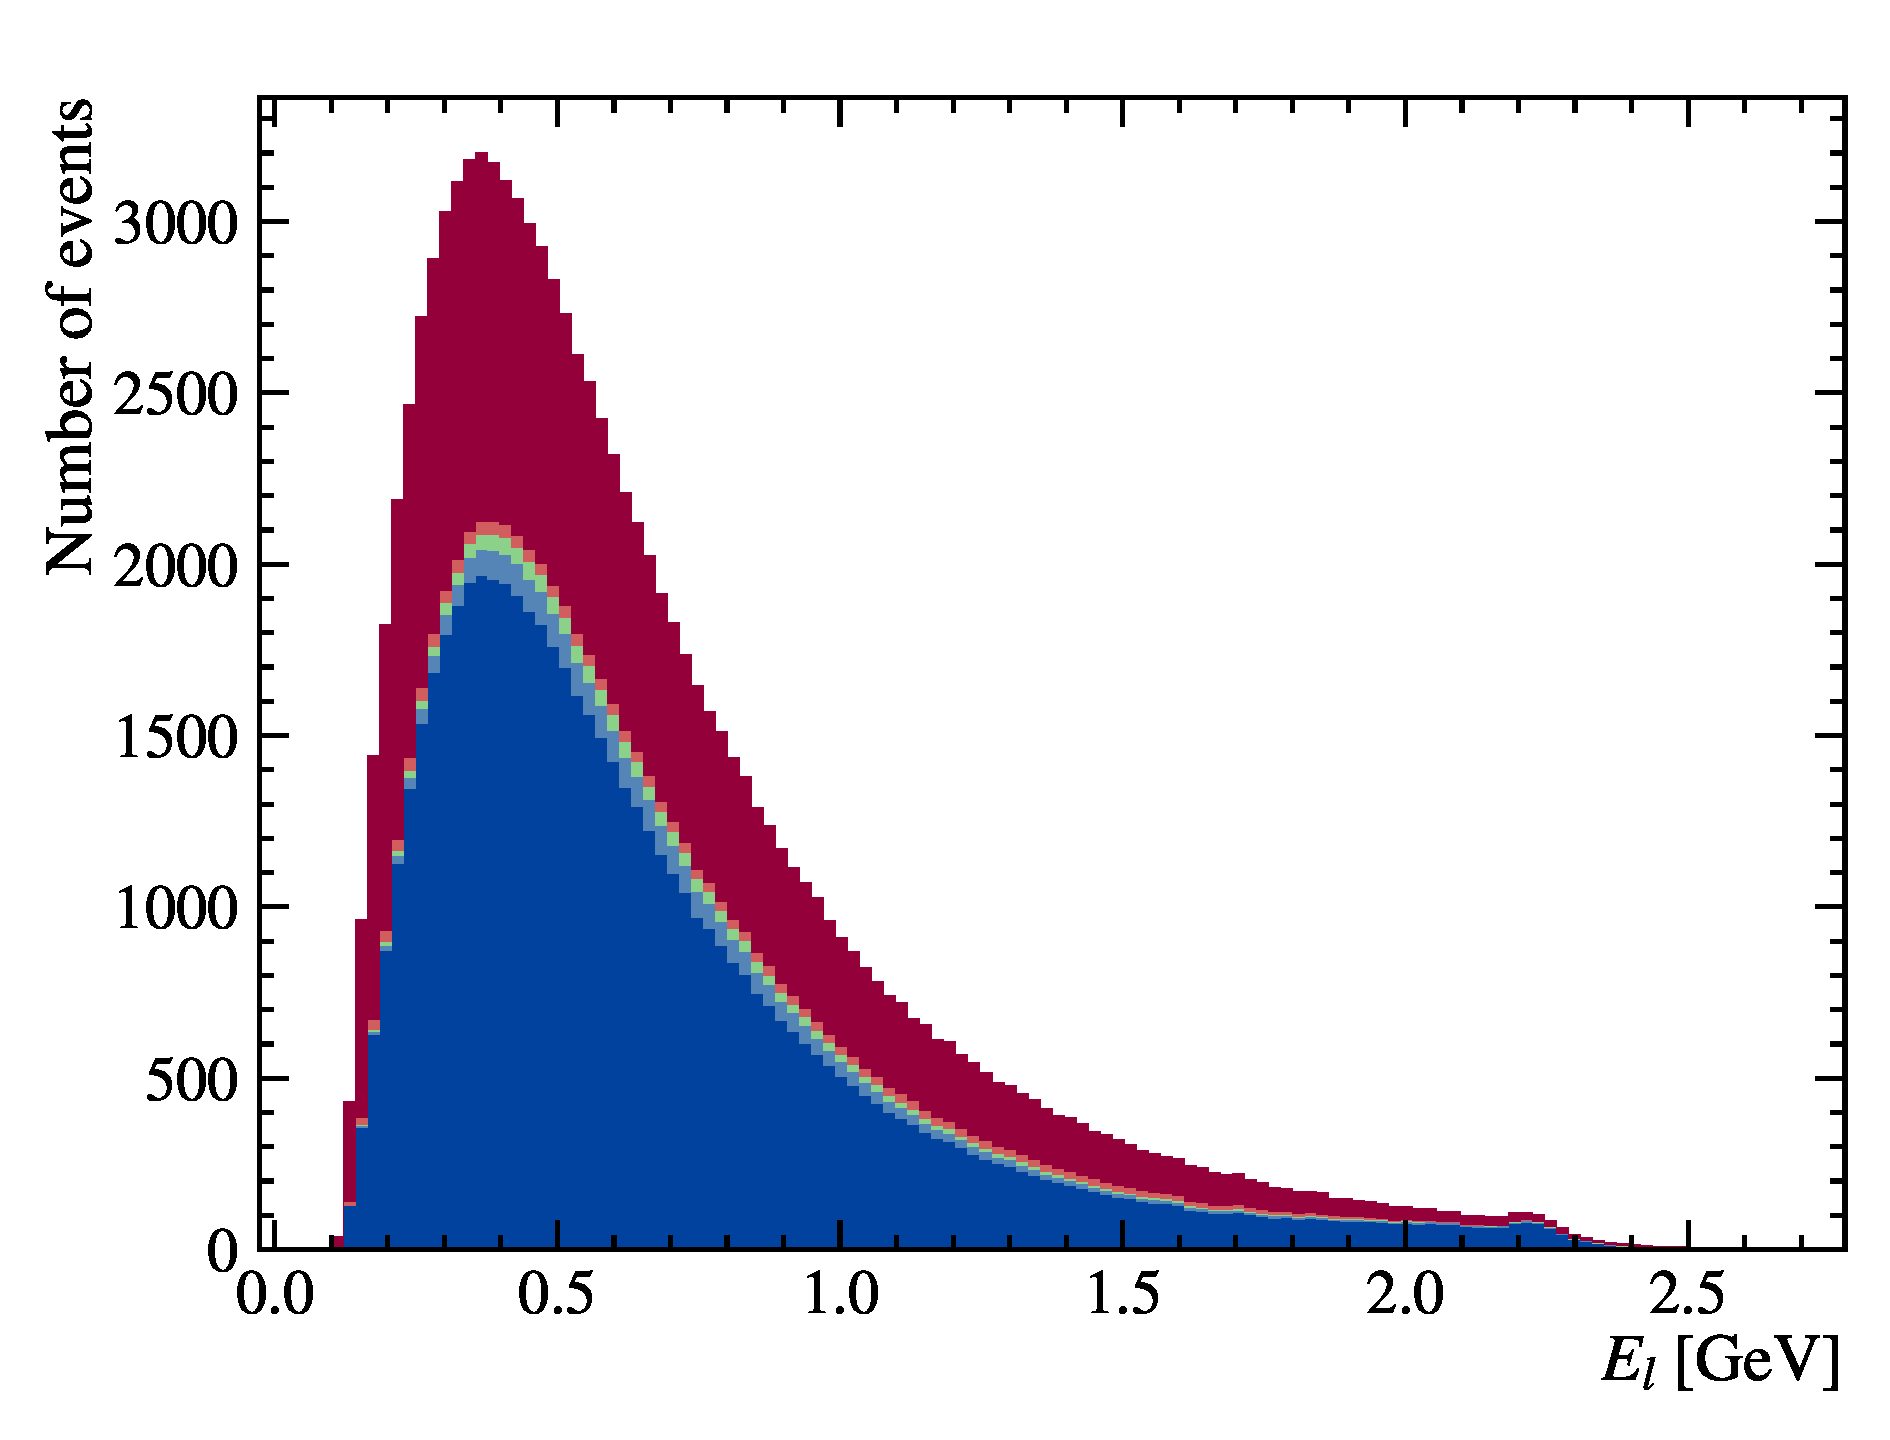
\includegraphics[width=\textwidth]{figs-fit-fit-templates/data-driven-plots/misid/D0_el.pdf}
    \end{subfigure}
    \hfill
    \begin{subfigure}[b]{0.32\textwidth}
        \centering
        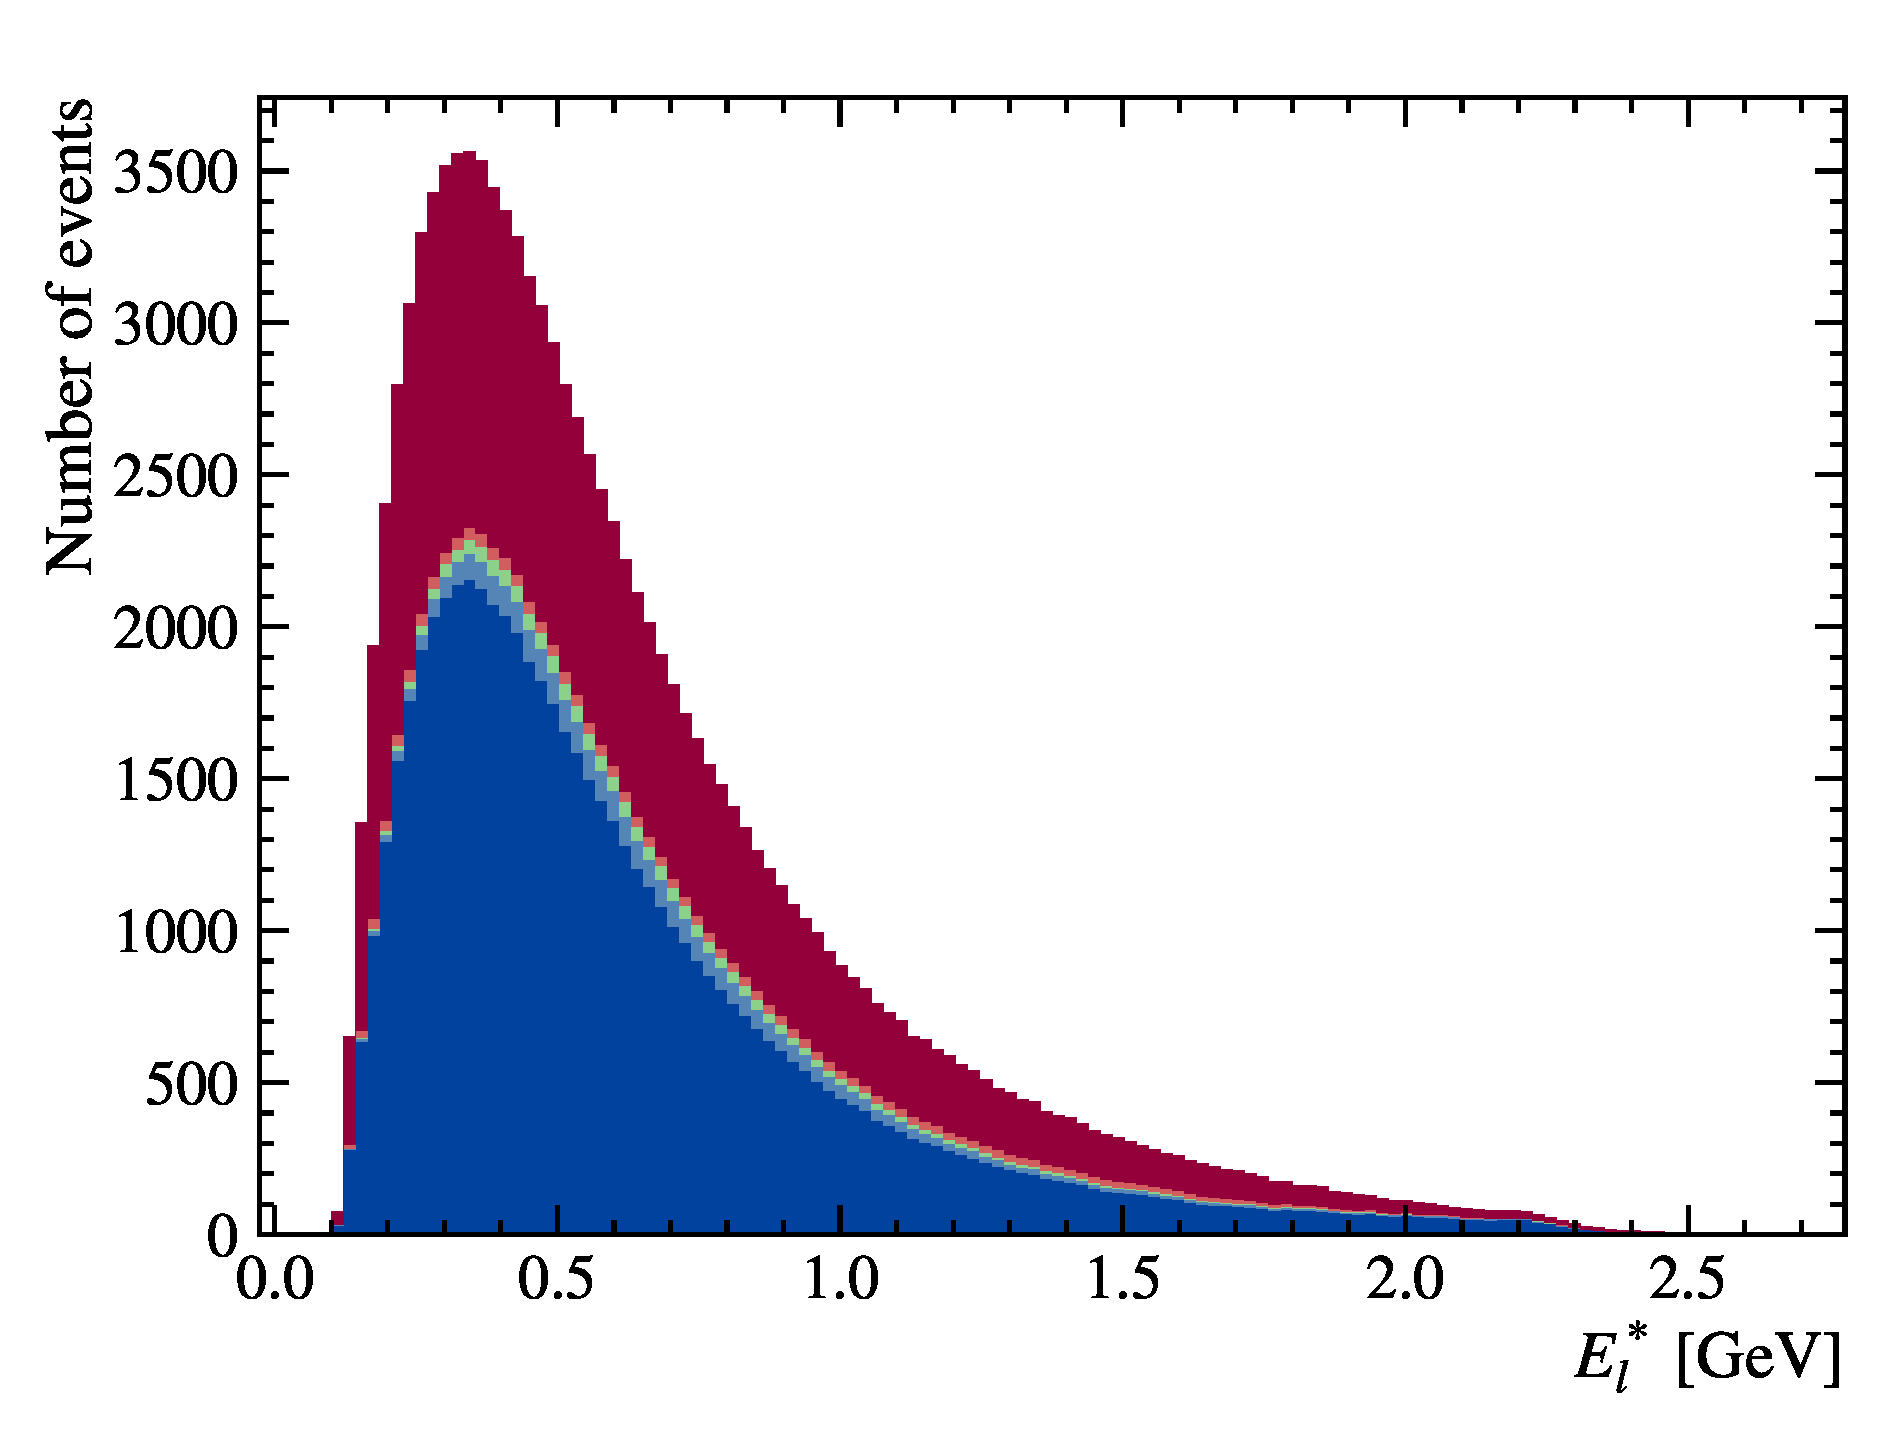
\includegraphics[width=\textwidth]{figs-fit-fit-templates/data-driven-plots/misid/D0_el_smr.pdf}
    \end{subfigure}
    \hfill
    \begin{subfigure}[b]{0.32\textwidth}
        \centering
        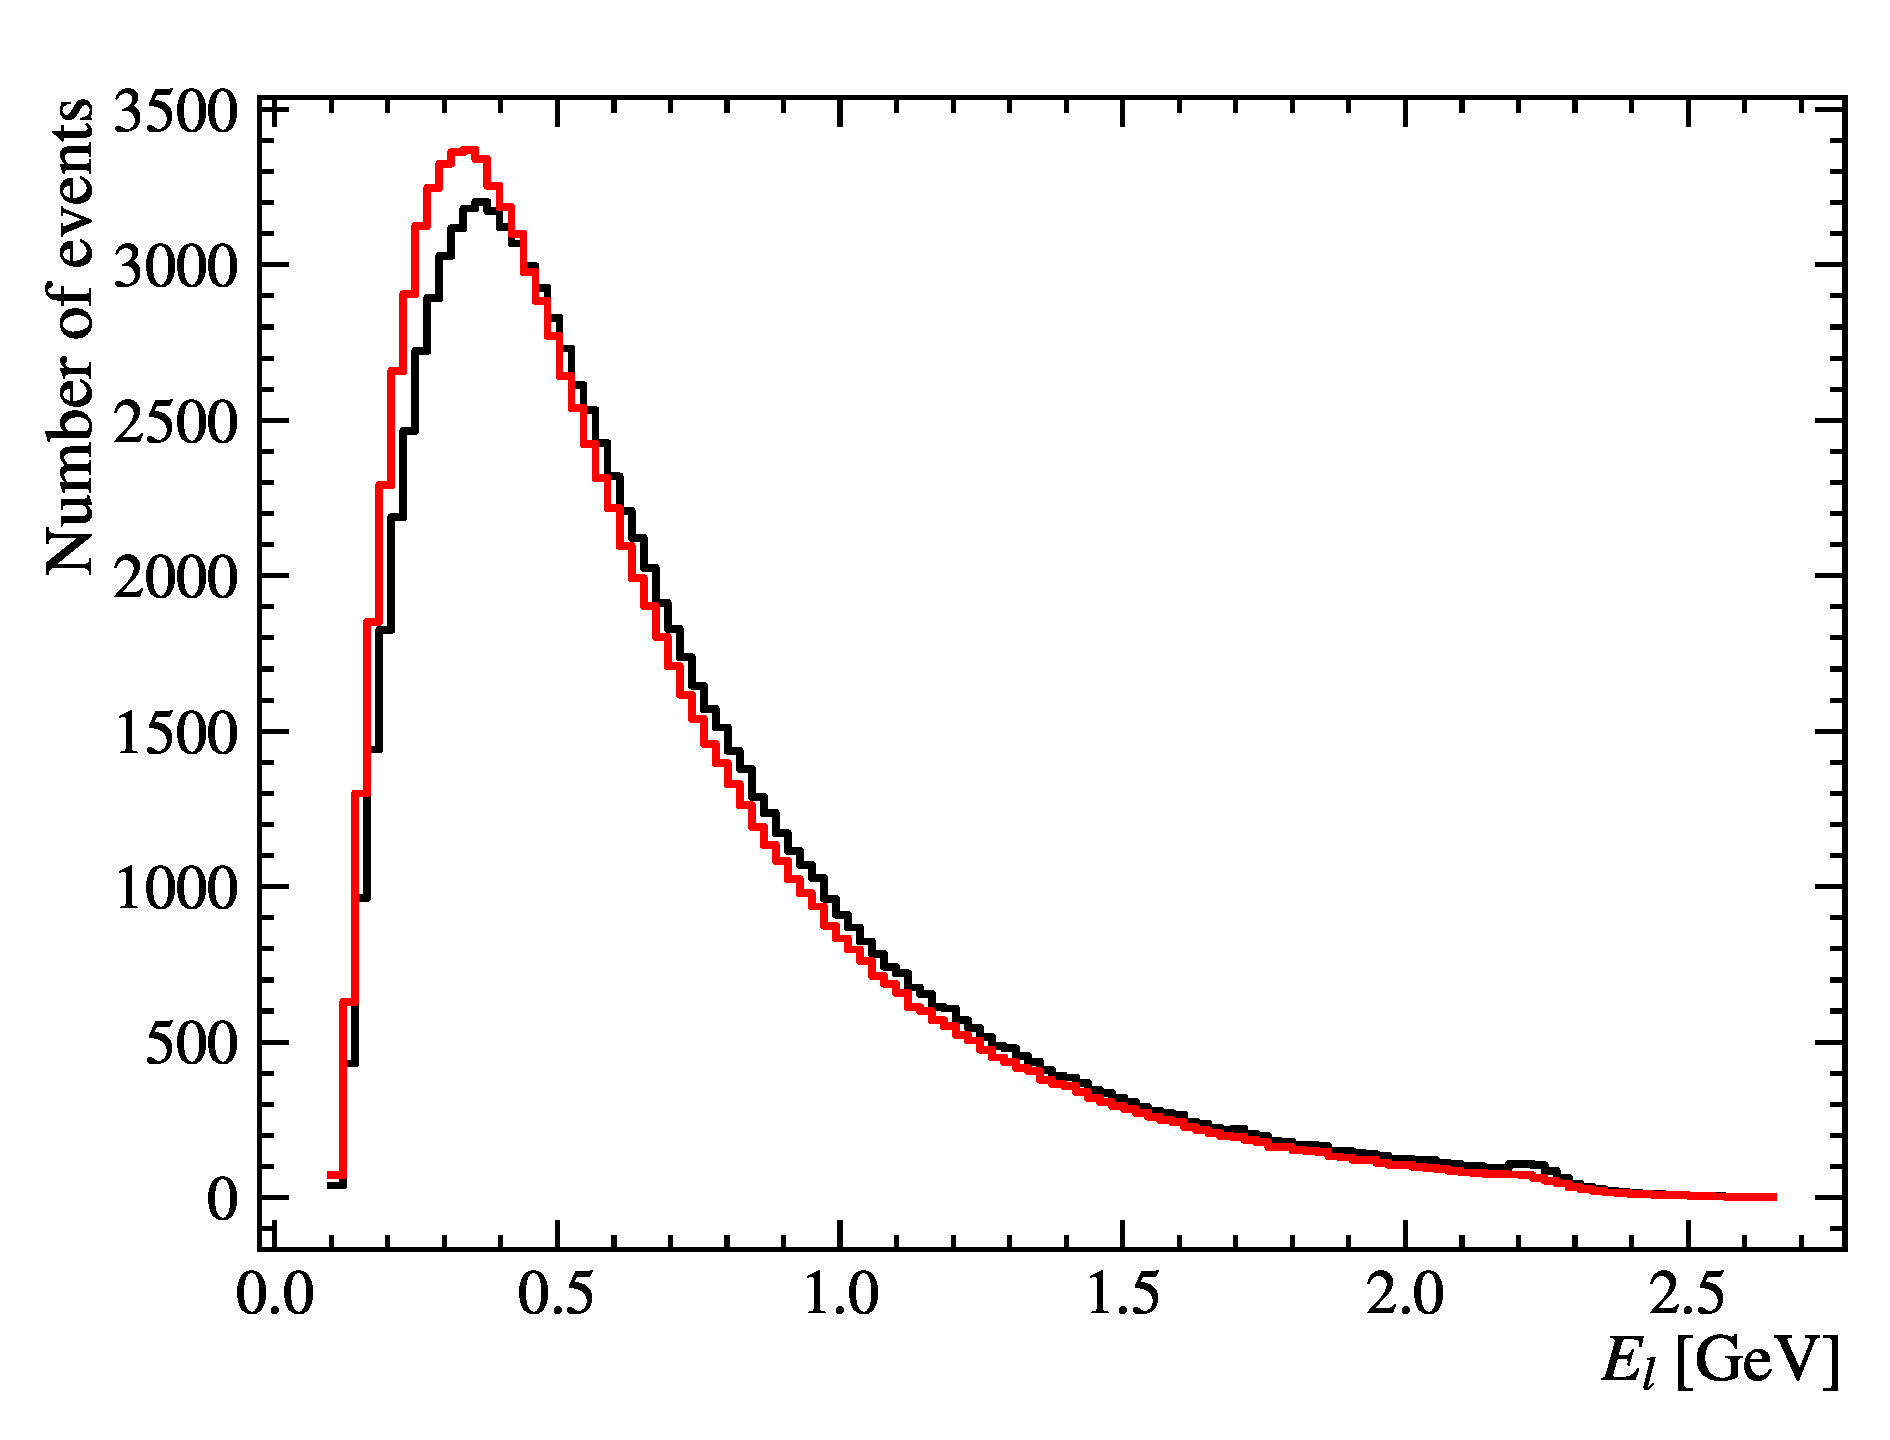
\includegraphics[width=\textwidth]{figs-fit-fit-templates/data-driven-plots/misid/D0_el_comp.pdf}
    \end{subfigure}
    \caption[Effect of DiF on fit variables]{
        Effect of DiF on fit variables.
        The plots displayed here are contributions of 2016 $D^0$ fake \muon
        control samples ($B^- \rightarrow D^0 t^-$) to the fit variables.

        The first column is unsmeared misID fit variables \mmSq, \qSq, \el; the
        second column smeared; the third column comparison between the overall
        shape of unsmeared/smeared fit variables.
        Note that the total number of events is not guaranteed to be conserved,
        because smearing may put fit variables outside of the
        acceptance range.
    }
    \label{fig:unfolding-fit-vars-smear}
\end{figure}
